\documentclass[a4paper]{article} 
\addtolength{\hoffset}{-2.25cm}
\addtolength{\textwidth}{4.5cm}
\addtolength{\voffset}{-3.25cm}
\addtolength{\textheight}{5cm}
\setlength{\parskip}{0pt}
\setlength{\parindent}{0in}

%----------------------------------------------------------------------------------------
%	PACKAGES AND OTHER DOCUMENT CONFIGURATIONS
%----------------------------------------------------------------------------------------
\usepackage{enumitem} 
\usepackage{blindtext} % Package to generate dummy text
\usepackage{charter} % Use the Charter font
\usepackage[utf8]{inputenc} % Use UTF-8 encoding
\usepackage{microtype} % Slightly tweak font spacing for aesthetics
\usepackage[english]{babel} % Language hyphenation and typographical rules
\usepackage{amsthm, amsmath, amssymb} % Mathematical typesetting
\usepackage{float} % Improved interface for floating objects
\usepackage[final, colorlinks = true, 
            linkcolor = black, 
            citecolor = black]{hyperref} % For hyperlinks in the PDF
\usepackage{graphicx, multicol} % Enhanced support for graphics
\usepackage{xcolor} % Driver-independent color extensions
\usepackage{marvosym, wasysym} % More symbols
\usepackage{rotating} % Rotation tools
\usepackage{censor} % Facilities for controlling restricted text
\usepackage{listings, style/lstlisting} % Environment for non-formatted code, !uses style file!
\usepackage{pseudocode} % Environment for specifying algorithms in a natural way
\usepackage{style/avm} % Environment for f-structures, !uses style file!
\usepackage{booktabs} % Enhances quality of tables
\usepackage{tikz-qtree} % Easy tree drawing tool
\tikzset{every tree node/.style={align=center,anchor=north},
         level distance=2cm} % Configuration for q-trees
\usepackage{style/btree} % Configuration for b-trees and b+-trees, !uses style file!
\usepackage[backend=biber,style=numeric,
            sorting=nyt]{biblatex} % Complete reimplementation of bibliographic facilities
\addbibresource{ecl.bib}
\usepackage{csquotes} % Context sensitive quotation facilities
\usepackage[yyyymmdd]{datetime} % Uses YEAR-MONTH-DAY format for dates
\renewcommand{\dateseparator}{-} % Sets dateseparator to '-'
\usepackage{fancyhdr} % Headers and footers
\pagestyle{fancy} % All pages have headers and footers
\fancyhead{}\renewcommand{\headrulewidth}{0pt} % Blank out the default header
\fancyfoot[L]{} % Custom footer text
\fancyfoot[C]{} % Custom footer text
\fancyfoot[R]{\thepage} % Custom footer text
\newcommand{\note}[1]{\marginpar{\scriptsize \textcolor{red}{#1}}} % Enables comments in red on margin

%----------------------------------------------------------------------------------------

\begin{document}
	
	%-------------------------------
	%	TITLE SECTION
	%-------------------------------
	
	\fancyhead[C]{}
	\hrule \medskip % Upper rule
	\begin{minipage}{0.295\textwidth} 
		\raggedright
		\footnotesize
		  Sharif University of Technology \hfill\\   
		Computer Engineering Department\hfill\\
		Sharifi-Azarkhalili
            %\begin{figure}
    	%	
\includegraphics{SharifEngLogo.png}
    	% \end{figure}
	\end{minipage}
	\begin{minipage}{0.4\textwidth} 
		\centering 
		\large 
		Homework Assignment 2\\ 
		\normalsize 
		Introduction to Machine Learning, Fall 2022\\ 
	\end{minipage}
	\begin{minipage}{0.295\textwidth} 
		\raggedleft
		\small
            1401-08-02
            \hfill\\
	\end{minipage}
	\medskip\hrule 
	\bigskip
	
	%-------------------------------
	%	CONTENTS
	%-------------------------------
        \begin{center}
            Alireza Gargoori Motlagh, Sina Mazaheri, Hadis Ahmadian, Taha Akbari
        \end{center}
        
        %-----------------------Question 1-------------------------
        
        \section{Clustering and K-means (35 points)}
    
        \subsection{Intuitive Understanding}
        \begin{itemize}
        \item In  each sample below, draw the boundry that $K$-means finds for $K=2$. Do you think the clusters separated by borders found by $K$ means is meaningfull in each case? If not, what property of data causes this?
        \end{itemize}
        \begin{center}
        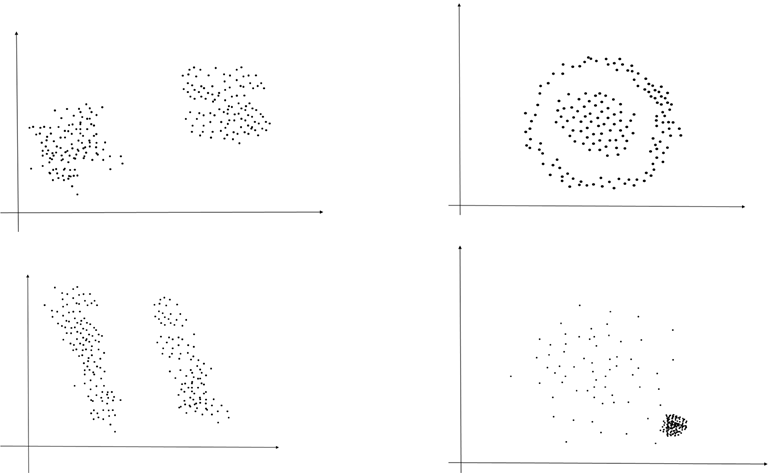
\includegraphics[scale=0.5]{Q1}
        \end{center}
        
        \begin{itemize}
        \item In which case above, feature scaling can solve the problem? Why?
        \end{itemize}
         
        \begin{subsection}{Finding proper value of $K$}
        \begin{center}
         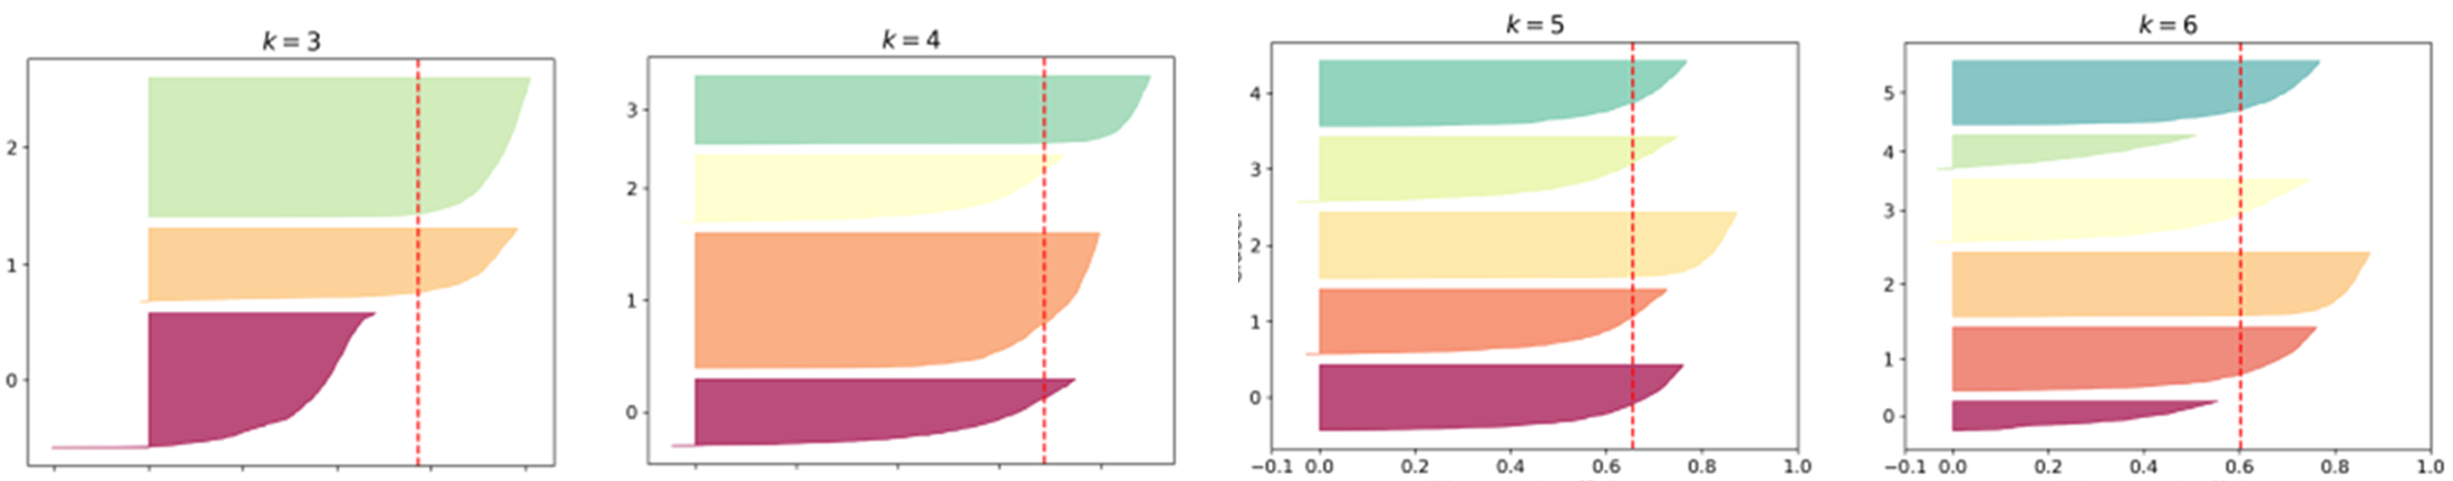
\includegraphics[scale=0.25]{Q1_B}
        \end{center}
        \begin{itemize}
        \item For finding a proper value for $K$, what is the advantage of using silhouette score in comparison to inertia?
        \item In the figure above, you can see silhouette diagram for different values of k. which value for $K$ is better? Why?
        \end{itemize}
        \subsection{Applications of Clustering}
        Two applications of clustering are Active learning and semi-supervised learning. Explain usage of clusting in each of these approaches and the diffrences between them briefly.
        \end{subsection}
        \bigskip
    
        %-----------------------Question 2-------------------------
        
        \section{Whitening Using PCA (25 points)}
        \textbf{Whitening} is one of the pre-processing techniques which is used in practical ML. By whitening, we mean that for a given feature matrix $\mathbf{X}$, this feature matrix should have zero mean vector and identity matrix as its covariance matrix. Explain that how we could transform $\mathbf{X}$ by using its covariance matrix principal components in order to have a whitened data set? After that, prove this new feature matrix has the desired properties, namely, zero mean vector and identity matrix as its covariance matrix.
        \bigskip
    
        %-----------------------Question 3-------------------------
        
        \section{Linear Regression}
        \subsection{Lagrange Multipliers (25 points)}
        Using Lagrange Multipliers give a geometric interpretation of why Lasso Regression results in more sparse solutions. Consider using $L_p $where $p<1$ instead of $p=1$. Show that we will get even more sparse solutions when we decrease $p$. Additionally explain why $L_1$ norm is used instead of smaller values for getting sparse solutions. (Hint: Analysis the convexity of unit ball with $L_p$ norm.)
        \subsection{Ridge Regression (optional) (10 points)} 
        Prove that the optimal value for the Ridge regression is $\mathbf{w}^{*} = (\mathbf{X}^{\top}\mathbf{X} + \lambda \mathbf{I})^{-1}\mathbf{X}^{\top}\mathbf{y}$ and can be obtained by minimizing the Error function below:
        \begin{align}
        L(\mathbf{w}) = \|\mathbf{X}\mathbf{w} - \mathbf{y}\|_{2}^{2} + \frac{1}{2}\lambda\|\mathbf{w}\|_{2}^{2}
        \end{align}
        \bigskip

        %-----------------------Question 4-------------------------
    
        \section{Generalization Error (15 points)}
        \begin{itemize}
        \item What is the effect of dimentionality reduction on overfitting? Why?
        \item We know that one solution for overfitting is using more data for training. However finding more data is not always possible, in this case we can alter the data that we already have so that by changing them slightly, we generate new data. This is called data augmentation. Search about data augmentation methods and give three examples of them.
        \end{itemize}
        \bigskip

        %-----------------------Question 5-------------------------
	\section{Kernels}
	\subsection{Feature Space (15 points)}
	Consider $x, y \in \mathbb{R}^2$, the kernel function defined as 
	$$k(x,y) = (1+cos\\
	(\angle x,y))^2 ,$$
	where $cos(\angle x,y)$ means the cosine of the angle between $x$ and $y$ vectors. Find the feature space $\phi(x)$ which corresponds to this kernel.
 
	\subsection{Kernel Matrix (20 points)}
	\subsubsection{}
	Suppose for now that $k$ is indeed a valid kernel corresponding to some
	feature mapping $\phi$. Now, consider some infinite set of m points, $\{x^{(1)},...,x^{(m)}\}$, and let a square m-by-m matrix $K$ be
	defined so that its $(i,j)$-entry is given by $K_{i,j} = k(x^{(i)}; x^{(j)})$. This matrix is called the Kernel matrix. 
	
	Prove that $K$ is a positive semi-definite matrix.
	
	\subsubsection{}
	The positive semi-definitivity of kernel matrix turns out to be not only a necessary, but also a sufficient, condition for $k$ to be a valid kernel, also called a Mercer kernel.
	
	Prove that if $K$(kernel matrix) is a positive semi-definite matrix, then $k$ is a dot product: $\exists \phi$ such that $k(x,y) = \phi(x).\phi(y)$
	
	(Hint: Use diagonalization for real symmetric matrices.)
	
	\bigskip
	
	%-----------------------Question 6-------------------------
	
	\section{Feature Expansion (20 points)}
	
	\subsection{}
	For each dataset below in figure 1, find a 1-dimensional transform $\phi: R^d \rightarrow R$ such that in the new feature space, 2 classes are linearly separable.
	\begin{figure}
		[hbt!]
		\centering
		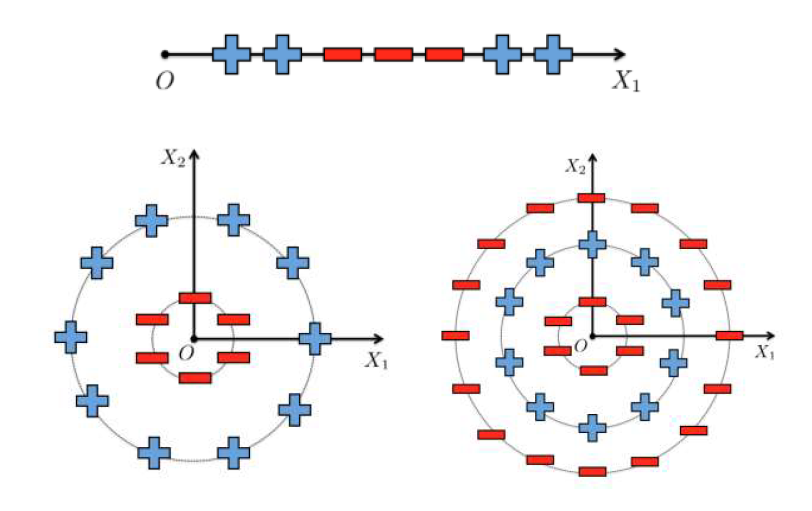
\includegraphics[scale=0.45]{Figure1.png}
		\caption{Datasets in original feature space}
	\end{figure}
	
	\subsection{}
	As you know, the equation of a circle in 2-d plane is defined as $(x_1 - a)^2 + (x_2 - b)^2 - r^2 = 0$. By expanding the former equation, show that any circular region is linearly separable in $(x_1, x_2, x_1^2, x_2^2)$ feature space.
	\bigskip
	
	%-----------------------Question 7-------------------------
	
	\section{SVM Decision Boundaries (30 points)}
	In Figure 2 we have plotted the decision boundaries and margins for SVM learned on the
	same data set using the following parameters (not in the same order as the figures):

	\begin{enumerate}[label=(\roman*)]
		\item Linear kernel, C = 0.1
		\item Linear kernel, C = 1
		\item Linear kernel, C = 10
		\item RBF kernel, $\gamma$ = 0.1, C = 15
		\item RBF kernel, $\gamma$ = 1, C = 3
		\item RBF kernel, $\gamma$ = 10, C = 1
	\end{enumerate}
	
	Match each one of the figures with one of these parameter settings. Explain your matchings in few sentences.

	\begin{figure}
		[hbt!]
		\centering
		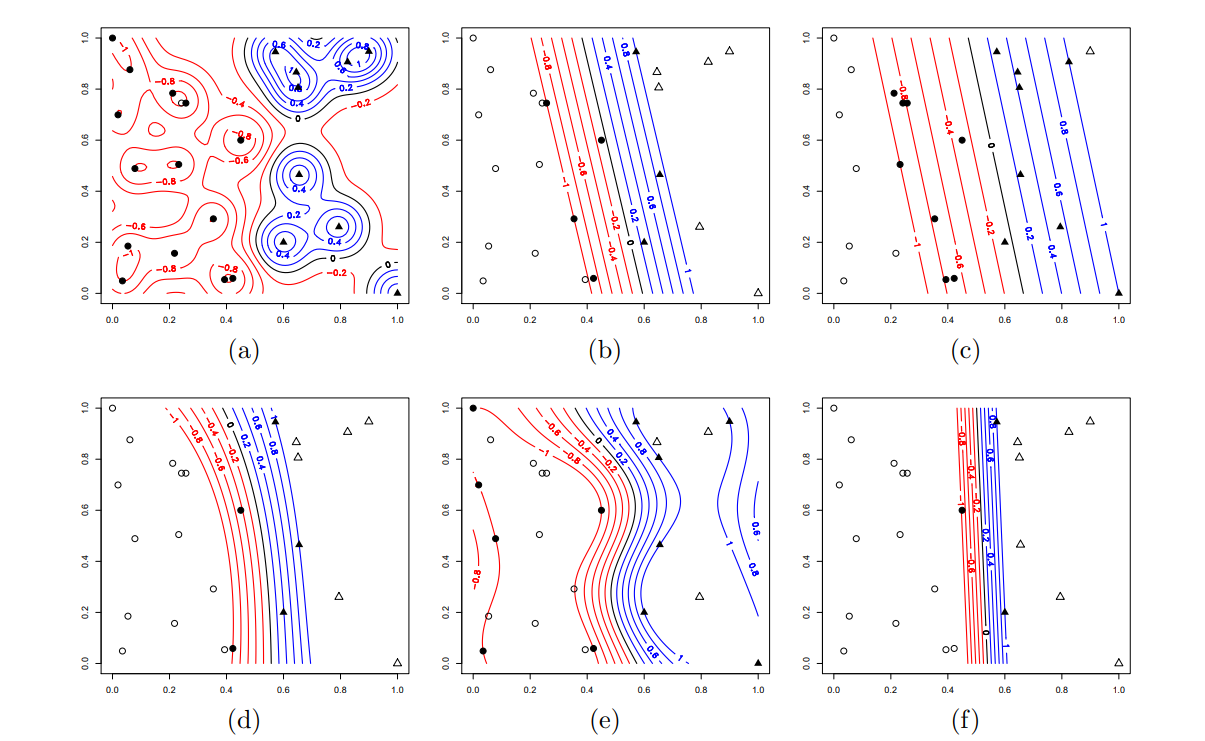
\includegraphics[scale=0.36]{Figure2.png}
		\caption{Circles and triangles denote Class 1 and 2 respectively, solid points are support vectors.}
	\end{figure}

        %-----------------------Question 8-------------------------
        \section{Monte Carlo Cross Validation (15 points)}
        In Monte Carlo Cross Validation(MCCV), also known as repeated random subsampling CV, you randomly select (without replacement) some fraction of your data to form the training set, and then assign the rest of the points to the validation set. This process is then repeated multiple times, generating (at random) new training and validation partitions each time. In other words, it simply splits the $N$ data points into the two subsets $n_t$ and $n_v$ by sampling, without replacement. There exists $N \choose n_t$ unique training sets, but MCCV avoids the need to run this many iterations.

        \subsection{}
        How does the choice of $n_t$ affects the bias-variance trade-off?
        \subsection{}
        Compare MCVV with k-Fold Cross Validation and state its pros and cons.
        
	
\end{document}
